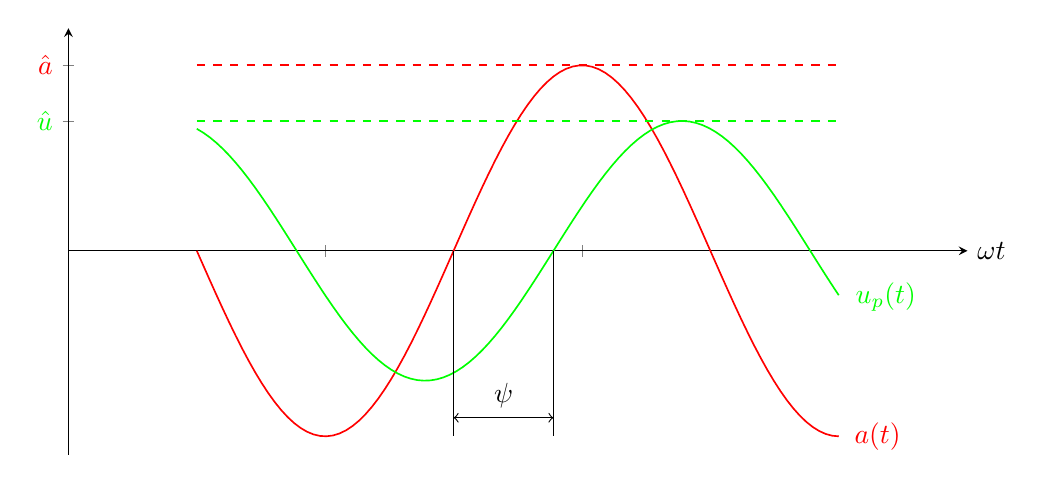
\begin{tikzpicture}
\begin{axis}[
    width=13cm, 
    height=7cm,
    axis x line=center, 
    axis y line=middle, 
    xlabel={$\omega t$},
     x label style={at={(current axis.right of origin)}, right},
    samples=100,
    ymin=-1.1, ymax=1.2,
    xmin=0, xmax=11,
    domain=0.5*pi:3*pi,
    xtick={   3.14159,  6.28318  },
    xticklabels={  ,  }, 
    ytick={0.7, 1},
    yticklabels={{\color{green}$\hat{u}$}, {\color{red} $\hat{a}$}}
]
\addplot [mark=none, semithick, red, dashed] {1};
\addplot [mark=none, semithick, red] {cos(deg(x))};
\addplot [mark=none, semithick, green, dashed] {0.7};
\addplot [mark=none, semithick, green] {0.7*cos(deg(x)-70)};
\node[text=red] at (axis cs: 9.9,-1.0) {$a(t)$};
\node[text=green] at (axis cs:10.0,-0.25) {$u_p(t)$};
\draw (axis cs: 4.712389, 0) -- (axis cs: 4.712389, -1);
\draw (axis cs: 5.934119, 0) -- (axis cs: 5.934119, -1);
\draw[<->] (axis cs: 4.712389, -0.9) -- node[above]{$\psi$} (axis cs: 5.934119, -0.9);
\end{axis}
\end{tikzpicture}
